\documentclass{article}
\usepackage{standalone}
\usepackage[catalan,english]{babel}
\usepackage{amsmath,amssymb,amsthm}
\usepackage[sorting=none,maxnames=10]{biblatex}
\usepackage[left=2.8cm,right=2.8cm,top=3cm,bottom=3cm]{geometry}
\usepackage[colorlinks,linkcolor=blue,citecolor=blue,urlcolor=blue]{hyperref}
\usepackage{stmaryrd,csquotes}
\usepackage[affil-it]{authblk}
\usepackage{multirow}
\usepackage{physics}
%%%%%%%%% more colors %%%%%%%%%%%%
\usepackage{xcolor}
\definecolor{darkblue}{RGB}{86, 40, 240}
\definecolor{lessgreen}{RGB}{0,100,0}
\definecolor{color1}{RGB}{255,158,1}
\definecolor{color2}{RGB}{255,74,1}
\definecolor{color3}{RGB}{220,0,0}
\usepackage[hypcap=false]{caption}
%%%%%%%%% tiks-picture %%%%%%%%%%%
\usepackage{tikz}
\usepackage{pgfplots}
\usepackage{mathtools}
\usetikzlibrary{patterns}
\pgfplotsset{compat = newest}
%%%%%%%%%%%%%%%%%%%%%%%%%%%%%%%%%%
\usepackage{subfig}
%%%%%%%%%%% Pels codis en C o Python que posarem en un annex %%%%%%%%%%
\usepackage{listings}

\renewcommand{\lstlistingname}{Programa}

\lstloadlanguages{C,Python,bash}
\lstset{ %
        backgroundcolor=\color{white},   % choose the background color; you must add \usepackage{color} or \usepackage{xcolor}
        basicstyle=\color{red}\footnotesize\ttfamily,        % the size of the fonts that are used for the code
        breakatwhitespace=false,         % sets if automatic breaks should only happen at whitespace
        breaklines=true,                 % sets automatic line breaking
        captionpos=b,                    % sets the caption-position to bottom
        deletekeywords={...},            % if you want to delete keywords from the given language
        escapeinside={\%*}{*)},          % if you want to add LaTeX within your code
        extendedchars=true,              % lets you use non-ASCII characters; for 8-bits encodings only, does not work with UTF-8
        frame=single,                    % adds a frame around the code
        keepspaces=true,                 % keeps spaces in text, useful for keeping indentation of code (possibly needs columns=flexible)
        keywordstyle=\color{darkblue},       % keyword style
        commentstyle=\itshape\color{gray},
        identifierstyle=\color{black},
        language=C,                 % the language of the code
        otherkeywords={*,...},           % if you want to add more keywords to the set
        numbers=left,                    % where to put the line-numbers; possible values are (none, left, right)
        numbersep=5pt,                   % how far the line-numbers are from the code
        numberstyle=\tiny\color{gray}, % the style that is used for the line-numbers
        rulecolor=\color{gray},         % if not set, the frame-color may be changed on line-breaks within not-black text (e.g. comments (green here))
        showspaces=false,                % show spaces everywhere adding particular underscores; it overrides 'showstringspaces'
        showstringspaces=false,          % underline spaces within strings only
        showtabs=false,                  % show tabs within strings adding particular underscores
        stepnumber=1,                    % the step between two line-numbers. If it's 1, each line will be numbered
        stringstyle=\color{blue},     % string literal style
        tabsize=2,                         % sets default tabsize to 2 spaces
        %title=\lstname                   % show the filename of files included with \lstinputlisting; also try caption instead of title
}
\lstset{literate=
        {á}{{\'a}}1 {é}{{\'e}}1 {í}{{\'i}}1 {ó}{{\'o}}1 {ú}{{\'u}}1
        {Á}{{\'A}}1 {É}{{\'E}}1 {Í}{{\'I}}1 {Ó}{{\'O}}1 {Ú}{{\'U}}1
        {à}{{\`a}}1 {è}{{\`e}}1 {ì}{{\`i}}1 {ò}{{\`o}}1 {ù}{{\`u}}1
        {À}{{\`A}}1 {È}{{\'E}}1 {Ì}{{\`I}}1 {Ò}{{\`O}}1 {Ù}{{\`U}}1
        {ä}{{\"a}}1 {ë}{{\"e}}1 {ï}{{\"i}}1 {ö}{{\"o}}1 {ü}{{\"u}}1
        {Ä}{{\"A}}1 {Ë}{{\"E}}1 {Ï}{{\"I}}1 {Ö}{{\"O}}1 {Ü}{{\"U}}1
        {â}{{\^a}}1 {ê}{{\^e}}1 {î}{{\^i}}1 {ô}{{\^o}}1 {û}{{\^u}}1
        {Â}{{\^A}}1 {Ê}{{\^E}}1 {Î}{{\^I}}1 {Ô}{{\^O}}1 {Û}{{\^U}}1
        {œ}{{\oe}}1 {Œ}{{\OE}}1 {æ}{{\ae}}1 {Æ}{{\AE}}1 {ß}{{\ss}}1
        {ű}{{\H{u}}}1 {Ű}{{\H{U}}}1 {ő}{{\H{o}}}1 {Ő}{{\H{O}}}1
        {ç}{{\c c}}1 {Ç}{{\c C}}1 {ø}{{\o}}1 {å}{{\r a}}1 {Å}{{\r A}}1
        {€}{{\EUR}}1 {£}{{\pounds}}1
}
%%%%%%%%%%%%%%%%%%%%%%%%%%%%%%%%%%%%%%%%%%%%%%%%%%%%

\theoremstyle{definition}
\newtheorem{definition}{Definició}[section]
\newtheorem{theorem}[definition]{Teorema}
\newtheorem{prop}[definition]{Proposició}
\newtheorem{lemma}[definition]{Lema}
\newtheorem{corollary}[definition]{Coro\lgem ari}

\newcommand\quot[2]{
    \mathchoice
        {% \displaystyle 
        \text{\raise1ex\hbox{$#1$}\!\Big/\!\lower1ex\hbox{$#2$}}}
        {% \textstyle
            #1/#2}
        {% \scriptstyle
            #1/#2}
        {% \scriptscriptstyle  
            #1/#2}
}% quotient group. Usage A/B--->\quot{A}{B}.

\newcommand{\0}{\ensuremath{\vb{0}}}
\newcommand{\X}{\ensuremath{\vb{X}}}
\newcommand{\Y}{\ensuremath{\vb{Y}}}
\newcommand{\Z}{\ensuremath{\vb{Z}}}
\newcommand{\NN}{\ensuremath{\mathbb{N}}} % set of real numbers
\newcommand{\RR}{\ensuremath{\mathbb{R}}} % set of real numbers
\newcommand\Hz{\text{ Hz}}
\DeclareMathOperator{\arccosh}{arccosh}

\addbibresource{references.bib}

%%% url symbol for references it is needed \usepackage{stmaryrd} %%%
\newcommand\enllas{\raise.5pt\hbox{$\boxempty\kern-4.85pt{}^{\nearrow}$}\kern-2pt}

\DeclareFieldFormat{url}{%
  \ifhyperref
    {\href{#1}{\enllas}}
    {\url{#1}}}
%%%%%%%%%%%%%%%%%%%%%%%%%%%%%%%%%%%%%%%%%%%%%%%%%%%%%%%%%%%%%%%%%%%%

%%Atenció salts de línia manuals:
    %1-Secció: Model per a sons simples basat en la banda crítica; Frase: A l’hora d’incorporar les amplituds a la fórmula vam pensar diverses implementacions,...


\title{\bfseries\large MESURES DE DISSONÀNCIA}

\author{Víctor Ballester Ribó, NIU:1570866\endgraf Oriol Bosquet Gallardo, NIU: 1571598\endgraf Carlo Sala Gancho, NIU: 1570775}
\date{\parbox{\linewidth}{\centering
  Taller de modelització\endgraf
  Grau en Matemàtiques\endgraf
  Universitat Autònoma de Barcelona\endgraf
  Juny de 2021}}
\begin{document}
\maketitle
\selectlanguage{english}
\begin{abstract}
    Per si voleu posar abstract. De moment serveix per posar comentaris. Carlo: jo crec que sí que cal abstract
    \begin{itemize}
        \item L'estructura del treball (posar newpages...) ja la decidirem al final.
        \item Una pregunta: què us agrada més, primer la bibliografia o l'annex? No sé quin se sol posar davant...
        \item Us agrada el sagnat? A vegades queda bé, i a vegades no. Carlo: no m'agrada el sagnat
    \end{itemize}
\end{abstract}
\selectlanguage{catalan}
\tableofcontents
\section{Teoria musical}
Aquest treball està molt estretament relacionat amb la música, en com els humans percebem els sons i, per extensió, en les notes musicals. És per això que ens cal per una petita incursió en la teoria musical per poder entendre correctament el sentit del nostre model.\par
És ben conegut per a tothom que hi ha combinacions de notes musicals que sonen \textit{bé} i d'altres que sonen \textit{malament}. Ara bé, què volen dir \textit{bé} i \textit{malament} en aquest context? Vegem ara dues definicions que ens ho aclariran:
\begin{definition}
Anomenem \textit{consonància} la qualitat de dos o més sons amb una relació de freqüències concreta, que sonen agradables a l'oïda humana.\par
Anomenem \textit{dissonància} la qualitat de dos o més sons amb una relació de freqüències concreta, que sonen poc agradables a l'oïda humana.
\end{definition}
Quedant-nos amb aquestes definicions, descriurem en la secció \ref{teoria_auditiva} del treball quin és el motiu pel qual hi ha combinacions de sons que no són agradables a l'oïda humana.\par
Seguim amb algunes definicions que ens seran útils per caracteritzar els sons:
\begin{definition}
Siguin $f, a \in \mathbb{R}$. Anomenem \textit{so simple} el parell $(f, a)$ on $f$ és la freqüència del so i $a$ és l'amplitud d'aquest so.
\end{definition}
\begin{definition}
Siguin $F, A\in\mathbb{R}^n$ vectors tals que $F=(f_1,\ldots, f_n)$ i $A=(a_1,\ldots, a_n)$. Anomenem \textit{so complex} el parell $\mathcal{S}:=(F, A)$ compost per una sèrie d'harmònics de freqüències $f_i$ d'amplitud $a_i$, on $f_i = f_1 \cdot i$ i anomenem $f_1$ freqüència fonamental del so, que també descriurem com a $f$.
\end{definition}
Si observem l'escala musical, veiem que hi ha únicament 12 noms de notes diferents\footnotemark\space que es van repetint seguint el mateix patró en tota l'escala. Cal observar també:
\footnotetext{Ens centrarem, d'ara en endavant, en l'escala musical occidental, composta per les notes DO, DO\#, RE, RE\#, MI, FA, FA\#, SOL, SOL\#, LA, LA\#, SI.}
\begin{prop}
  Siguin $N_1, N_2$ dues notes musicals que tenen el mateix nom de nota i siguin $f_1, f_2$ les seves respectives freqüències fonamentals. Sense pèrdua de generalitat, suposem que $f_1 \leq f_2$. Llavors $\frac{f_{2}}{f_{1}} = 2^i$ per algun $i \in \mathbb{N}\cup\{0\}$.
\end{prop}
Per poder fer que això passi, es declara que la relació entre les freqüències de dues notes successives sempre és de $\sqrt[12]{2}$\footnotemark\space. D'aquesta manera, com que hem dit que hi ha 12 notes diferents, quan tornem a arribar a una nota amb el mateix nom que l'original haurem fet 12 salts de nota, és a dir, $\sqrt[12]{2}^{12} = 2$. Si fem aquests 12 salts $n$ vegades tindríem $\sqrt[12]{2}^{12\cdot n} = 2^n$ i, fem que es compleixi la proposició anterior.
\footnotetext{Aquesta manera de definir la distància entre notes de manera que totes les notes siguin equidistants entre si s'anomena Temperament igual \cite{wikitemp}.}
\section{Teoria auditiva}\label{teoria_auditiva}
El nostre cos ha desenvolupat un sistema complex per al reconeixement de sons fruit de milers d'anys d'evolució. Això juntament amb l'efecte de la cultura en la nostra vida ha provocat que un cert conjunt de freqüències sigui més agradable per a la nostra oïda que unes altres. Per tal de modelar en detall com percebem la dissonància, ens caldrà fer menció de dos conceptes clau en el sistema auditiu humà: la còclea i la membrana basilar. \par
La còclea és una estructura en forma de tub enrotllat en espiral, similar a la closca d'un caragol. Al centre i interior del tub s'hi troba una membrana anomenada membrana basilar (veure figura \ref{coclea}). Aquesta membrana vibra quan ones de so arriben a ella. Sobre la membrana basilar s'hi troba l'òrgan de Corti, que és el responsable de transformar les vibracions del so en impulsos nerviosos que són enviats al cervell.\par
Un concepte que serà important de cara a la caracterització del nostre model és el de banda crítica. Aquesta és l'amplada de freqüències dins de la qual un segon so interferirà amb la percepció d'un primer so en el sentit que activaran les mateixes cè\lgem ules de l'òrgan de Corti. Dit d'una altra manera, quan una freqüència arriba a la membrana basilar, aquesta fa que s'activin els receptors corresponents a aquesta freqüència i els receptors en un entorn (la banda crítica) d'aquesta. Per tant, si dues freqüències arriben a la membrana basilar i no són prou distants entre si, es produeix una interferència que fa que no siguem capaços de distingir cada freqüència per separat: es produeix dissonància. En canvi, si estan prou allunyades entre si, el nostre cervell les interpreta com a diferents i provoca una resposta agradable: es produeix consonància (veure figura \ref{membrana}).\par
\begin{figure}
    \begin{minipage}[c]{0.49\linewidth}
        \centering
        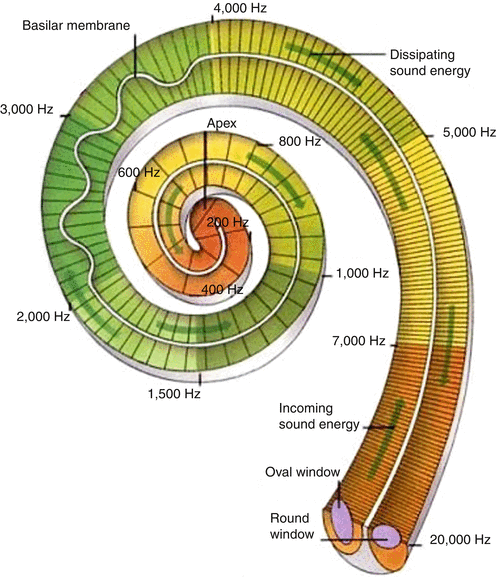
\includegraphics[height=0.6\linewidth]{Imatges_beamer2/coclea.png}
        \caption{Estructura de la còclea}
        \label{coclea}
    \end{minipage}
    \hfill
    \begin{minipage}[c]{0.49\linewidth}
        \centering
        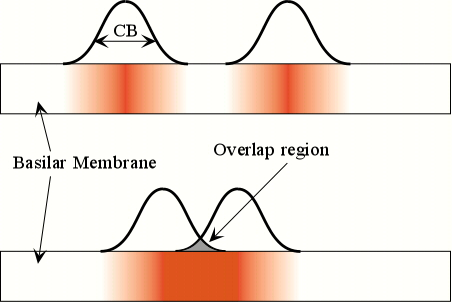
\includegraphics[height=0.6\linewidth]{Imatges_beamer2/basilar_membrane.jpg}
        \caption{Interferència de dos sons en la mem\-bra\-na basilar}
        \label{membrana}
    \end{minipage}
\end{figure}
Això ens porta a concloure que dues freqüències les percebem com a dissonants si es troben dins la mateixa banda i consonants si es troben en bandes diferents. \par
Hi ha diversos models que parametritzen l'amplada de banda crítica corresponent a cada freqüència de l'espectre audible. El més adient pel nostre model és el donat per William Hutchinson i Leon Knopoff en \cite{hutchinson} basat en dades de \cite{plomp,goodwin,mayer} que parametritza l'amplada de banda crítica amb la funció:
\begin{equation}
    \text{CBW}(f)=1.72 f^{0.65}
    \label{CBW}
\end{equation}
\section{Model per a sons simples basat en els batiments}
Per començar, farem un model per a sons purs o simples, és a dir, sons compostos per una sola freqüència i amplitud. Aquest primer model l'enfocarem des del punt de vista dels batiments. Per entendre què són exactament els batiments, comencem considerem dos sons sinusoïdals de diferent freqüència però mateixa amplitud: $$y_1(t)=A\sin(2\pi f_1 t),\qquad y_2(t)=A\sin(2\pi f_2 t).$$
Si fem la superposició dels dos sons obtenim: $$y(t)=y_1(t)+y_2(t)=2A\cos\left(2\pi\frac{f_1-f_2}{2}t\right)\sin\left(2\pi\frac{f_1+f_2}{2}t\right).$$
D'aquesta expressió podem observar dos freqüències diferents: $\frac{f_1-f_2}{2}$ i $\frac{f_1+f_2}{2}$. El sentit físic de la segona és la freqüència en què osci\lgem a l'amplitud de l'ona resultant. Aquesta ona ve modulada per una altra la qual vibra amb una freqüència igual a $\frac{f_1-f_2}{2}$ (vegeu figura \ref{main:fig1}). Si les dues freqüències estan suficientment a prop perquè la diferència $f_p:=|f_1-f_2|$ sigui petita, es creen els batiments: sons polsants (a freqüència $f_p$) interpretats a una sola freqüència corresponent a la mitjana de les dues inicials, és a dir, a $\frac{f_1+f_2}{2}$. A aquesta freqüència $f_p$ se la coneix com freqüència de pulsació. Si les dues freqüències estan molt separades, $f_p$ serà gran i, per tant, no es percebran els batiments i es podran distingir les dues freqüències amb claredat. Finalment, si les dues freqüències estan massa a prop per distingir-se amb claredat, però massa lluny per interpretar-se com una de sola es produirà el fenomen de dissonància.
\begin{center}
    \includestandalone[mode=image|tex,width=0.5\linewidth]{Imatges_main/sin}
    \captionof{figure}{Superposició de dues ones sinusoïdals amb equacions $y_1(t)=\sin(2\pi f_1 t)$ i $y_2(t)=\sin(2\pi f_2 t)$}
    \label{main:fig1}
\end{center}
Segons dades de \cite{gibson} els batiments creen dissonància quan aproximadament tenim $15\text{ Hz}<f_p<60\text{ Hz}$. Més precisament,
\begin{itemize}
    \item Si $f_p<10\text{ Hz}$: Interpretem un únic so i podem distingir els batiments.
    \item Si $15\text{ Hz}<f_p<60\text{ Hz}$: Els sons estan massa separats per ser interpretats com un de sol, però massa junts per distingir-se amb claredat. Es produeix dissonància.
    \item Si $f_p>60\text{ Hz}$: Podem distingir els dos sons amb claredat.
\end{itemize}
Empíricament hem comprovat que la màxima dissonància es troba a aproximadament 38 Hz de diferència d'una freqüència fixe al volant de 300 Hz. És a dir, donada una freqüència $f_1$ suposarem que la màxima dissonància entre $f_1$ i una altra freqüència $f_2>f_1$ es troba quan $f_2-f_1=38\text{ Hz}$. A més, prendrem les amplituds de les ones constants i iguals a 1, és a dir, $A=1$.\par Així doncs busquem una funció $\delta(f_1,f_2)$ que creixi monòtonament des de 0 fins un valor i a partir de llavors decreixi monòtonament de nou fins a 0. Aquesta funció serà la que valori el grau de dissonància entre els dos sons simples de freqüències $f_1$ i $f_2$. Per això hem escollit funcions de la forma $\cosh\left(ax^2\right)$ i $e^{-bx}$ per representar la dissonància en aquests dos intervals, on $x=\frac{f_2-f_1}{f_1}$ és la freqüència normalitzada. Si pressuposem que la maxima dissonància la tenim en el punt $x=\frac{38}{f_1}$, com hem mencionat anteriorment, i volem que assoleixi un valor de 1 en aquest punt, aleshores l'exponencial decreixent ha de ser de la forma $e^{-b\left(x-38/f_1\right)}$. Com que en aquest model la dissonància entre dues freqüències només depèn de la diferència entre aquestes, tenim que necessàriament s'ha de complir $b\propto f_1$. Per tant, $e^{-\beta f_1(x-38/f_1)}$, on hem escollit $\beta=0.15$ per obtenir uns resultats coherents.\par Pel que fa l'altra part de la funció $\delta(f_1,f_2)$ (la del creixement fins al valor màxim), similarment a com hem raonat anteriorment, la funció $\cosh\left(ax^2\right)$ ha de ser en realitat de l'estil $\cosh\left(ax^2\right)-1$ i com que, per sentit comú\footnote{És clar que al escoltar dues freqüències, una de les quals està fixada i l'altra és variable, no existeix un moment en què percebem un salt brusc en la interpretació del so resultant mentre variem la segona freqüència. Per tant, la funció de dissonància ha de ser necessàriament contínua.}, la funció de dissonància ha de ser contínua obtenim que en el punt $x=\frac{38}{f_1}$ la funció ha de valdre 1. Així doncs, hem de resoldre l'equació següent per trobar el valor de $a$ adequat:
$$\cosh\left[a\left(\frac{38}{f_1}\right)^2\right]-1=1.$$ Aquesta equació té solució quan $a=\arccosh(2)\left(\frac{f_1}{38}\right)^2$ i d'aquesta manera la funció en l'interval de creixement resulta ser: $$\cosh\left(\arccosh(2)\left(\frac{f_1}{38}\right)^2x^2\right).$$ Notem que, de nou, el valor només depèn de la diferència de freqüències $f_2-f_1$.\par Si anomenem $\gamma_{f_1}:=\frac{38}{f_1}$ tenim que la funció final de dissonància $\delta(f_1,f_2)$ és: $$\delta(f_1,f_2)=
    \left\{\begin{array}{lll}
        \cosh\left[\frac{\arccosh(2)}{\left(\gamma_{f_1}\right)^2}\left(\frac{f_2-f_1}{f_1}\right)^2\right]-1 & \text{si} & 1<\frac{f_2}{f_1}<1+\gamma_{f_1}\vspace{5pt}\\
        e^{-\beta f_1\left(\frac{f_2-f_1}{f_1}-\gamma_{f_1}\right)} & \text{si} & 1+\gamma_{f_1}<\frac{f_2}{f_1}
    \end{array}\right.$$ on $\beta=0.15$.
A la figura \ref{main:fig2} es mostra una representació d'aquesta fórmula.
\begin{center}
    \includestandalone[mode=image|tex,width=0.5\linewidth]{Imatges_main/model1}
    \captionof{figure}{Representació de la funció $\delta(f_1,f_2)$ a partir de varies freqüències base $f_1$ i fent variar $f_2$ o, més ben dit, fent variar $\frac{f_2}{f_1}$ suposant $f_2>f_1$.}
    \label{main:fig2}
\end{center}
És clar que el model descrit no diferencia si estem comparant dues freqüències prop dels 200 Hz o dues freqüències prop dels 2000 Hz. Només té en compte la diferència entre ambdues. Aquest és un primer inconvenient que podem trobar al model. Un segon problema podria ser que la corba té un punt on no és diferenciable (el màxim de la funció), cosa que ens porta a pensar si realment percebem els sons d'aquesta manera o d'una manera més suau, més \textit{diferenciable}. Aquests dos problemes ens porten a reconsiderar el problema inicial de calcular la dissonància entre dos sons purs i enfocar-ho des d'un altre punt de vista, com veurem a la secció següent.

\section{Model}
Com hem comentat anteriorment, distingirem dos tipus de sons: els sons simples i els sons complexos. Per això, ens anirà bé definir els següents conjunts:
\begin{definition}
    Definim el conjunt $\mathcal{S}$ de sons simples com: $$\mathcal{S}=\{s=(f,a,\varphi)\in\RR^3:f\in(0,\infty),a\in[0,\infty),\varphi\in[0,2\pi)\text{ i $s$ és el so d'equació }y_s(t)=a\sin(2\pi ft+\varphi)\}.$$
\end{definition}
\begin{definition}
    Definim el conjunt $\mathcal{C}$ de sons complexos com:
    \begin{multline*}
        \mathcal{C}=\Bigg\{\X=\{s_1,s_2,\ldots,s_3\}:s_i=(f_i,a_i,\varphi_i)\in\mathcal{S}\text{ per } i=1,\ldots,n\text{ i $\X$ és el so d'equació}\\y_{\X}(t)=\sum_{i=1}^ny_{s_i}(t)=\sum_{i=1}^na_i\sin(2\pi f_it+\varphi_i)\Bigg\}.
    \end{multline*}
\end{definition}
És a dir, el conjunt $\mathcal{C}$ està format per un conjunt de tuples de 3 elements (correponent a sons simples).\par
% A partir d'aquestes dues definicions observem que $\mathcal{S}\subset\mathcal{C}$. Definim ara la següent relació:
% \begin{definition}
%     Considerem el conjunt $\mathcal{C}$ i dos sons $\X,\Y\in\mathcal{C}$ definits per:
%     \begin{gather*}
%         \X=
%         \begin{pmatrix}
%             f_1 & \cdots & f_1 & f_2 & \cdots & f_2 & \cdots & f_n & \cdots & f_n\\
%             a_1 & \cdots & a_{r_1} & a_{r_1+1} & \cdots & a_{r_2} & \cdots & a_{r_{n-1}+1} & \cdots & a_{r_n}\\
%             \varphi_1 & \cdots & \varphi_1 & \varphi_2 & \cdots & \varphi_2 & \cdots & \varphi_n & \cdots & \varphi_n
%         \end{pmatrix},\\ \Y=
%         \begin{pmatrix}
%             g_1 & \cdots & g_1 & g_2 & \cdots & g_2 & \cdots & g_m & \cdots & g_m\\
%             b_1 & \cdots & b_{s_1} & b_{s_1+1} & \cdots & b_{s_2} & \cdots & b_{s_{m-1}+1} & \cdots & g_{s_m}\\
%             \phi_1 & \cdots & \phi_1 & \phi_2 & \cdots & \phi_2 & \cdots & \phi_m & \cdots & \phi_m
%         \end{pmatrix},
%     \end{gather*}
%     tals que $(f_i,\varphi_i)=(f_j,\varphi_j)\text{ i }(g_i,\phi_i)=(g_j,\phi_j)\iff i=j$; $f_i<f_j$ i $g_i<g_j$ si $i<j$, i $r_0=s_0:=0$. Observem que per la definició de sons complexos això ho podem suposar. Definim la relació $\sim$ com: $$\X\sim \Y\iff n=m\text{ i } \sum_{j=1}^{r_i}a_{r_{i-1}+j}=\sum_{j=1}^{s_i}b_{s_{i-1}+j}\quad\forall i=1,\ldots,n.$$
% \end{definition}
% \begin{lemma}
%     La relació $\sim$ és una relació d'equivalència.
% \end{lemma}
% \begin{proof}
%     Hem de veure comprovar les tres propietats que tenen les relacions d'equivalència. Per a tot $\X,\Y,\Z\in\mathcal{C}$ de la forma:
%     \begin{gather*}
%         \X=
%         \begin{pmatrix}
%             f_1 & \cdots & f_1 & f_2 & \cdots & f_2 & \cdots & f_n & \cdots & f_n\\
%             a_1 & \cdots & a_{r_1} & a_{r_1+1} & \cdots & a_{r_2} & \cdots & a_{r_{n-1}+1} & \cdots & a_{r_n}\\
%             \varphi_1 & \cdots & \varphi_1 & \varphi_2 & \cdots & \varphi_2 & \cdots & \varphi_n & \cdots & \varphi_n
%         \end{pmatrix},\\ \Y=
%         \begin{pmatrix}
%             g_1 & \cdots & g_1 & g_2 & \cdots & g_2 & \cdots & g_m & \cdots & g_m\\
%             b_1 & \cdots & b_{s_1} & b_{s_1+1} & \cdots & b_{s_2} & \cdots & b_{s_{m-1}+1} & \cdots & g_{s_m}\\
%             \phi_1 & \cdots & \phi_1 & \phi_2 & \cdots & \phi_2 & \cdots & \phi_m & \cdots & \phi_m
%         \end{pmatrix},\\\Z=
%         \begin{pmatrix}
%             h_1 & \cdots & h_1 & h_2 & \cdots & h_2 & \cdots & h_p & \cdots & h_p\\
%             c_1 & \cdots & c_{t_1} & c_{t_1+1} & \cdots & c_{t_2} & \cdots & c_{t_{p-1}+1} & \cdots & c_{t_p}\\
%             \psi_1 & \cdots & \psi_1 & \psi_2 & \cdots & \psi_2 & \cdots & \psi_p & \cdots & \psi_p
%         \end{pmatrix},
%     \end{gather*}
%     tals que $(f_i,\varphi_i)=(f_j,\varphi_j),(g_i,\phi_i)=(g_j,\phi_j)\text{ i }(h_i,\psi_i)=(h_j,\psi_j)\iff i=j$; $f_i<f_j$, $g_i<g_j$ i $h_i<h_j$ si $i<j$, i $r_0=s_0=t_0:=0$. Llavors es compleix:
%     \begin{enumerate}
%         \item Reflexivitat: $\X\sim \X$.\par És clar que es compleix.
%         \item Simetria: $\X\sim \Y\implies \Y\sim \X$.\par
%         \begin{multline*}
%             \X\sim \Y\implies n=m\text{ i } \sum_{j=1}^{r_i}a_{r_{i-1}+j}=\sum_{j=1}^{s_i}b_{s_{i-1}+j}\quad\forall i=1,\ldots,n\implies\\\implies m=n\text{ i }\sum_{j=1}^{s_i}b_{s_{i-1}+j}=\sum_{j=1}^{r_i}a_{r_{i-1}+j}\quad\forall i=1,\ldots,m\implies \Y\sim \X.
%         \end{multline*}
%         \item Transitivitat: $\X\sim \Y\text{ i }\Y\sim \Z\implies \X\sim \Z$:
%         \begin{multline*}
%             \left.
%             \begin{array}{l}
%                 \X\sim \Y\implies n=m\text{ i } \sum_{j=1}^{r_i}a_{r_{i-1}+j}=\sum_{j=1}^{s_i}b_{s_{i-1}+j}\quad\forall i=1,\ldots,n\\
%                 \Y\sim \Z\implies m=p\text{ i } \sum_{j=1}^{s_i}b_{s_{i-1}+j}=\sum_{j=1}^{t_i}a_{t_{i-1}+j}\quad\forall i=1,\ldots,m
%             \end{array}\right\}\implies\\\implies n=p\text{ i } \sum_{j=1}^{r_i}a_{r_{i-1}+j}=\sum_{j=1}^{t_i}b_{t_{i-1}+j}\quad\forall i=1,\ldots,n\implies \X\sim \Z.
%         \end{multline*}
%     \end{enumerate}
% \end{proof}
% \begin{definition}
%     Considerem el conjunt $\mathcal{C}$ amb la relació d'equivalència $\sim$. Definim la classe d'equivalència de $\X\in\mathcal{C}$ sota la relació $\sim$ com: $$\overline{\X}=\{\Y\in\mathcal{M}:\X\sim \Y\}.$$
% \end{definition}
% Observem que un representant natural de $\overline{\X}$ és $$
% \begin{pmatrix}
%     f_1 & \cdots & f_n\\
%     a_1 & \cdots & a_n\\
%     \varphi_1 & \cdots &\varphi_n
% \end{pmatrix}$$ on $(f_i,\varphi_i)=(f_)$
% \begin{definition}
%     Considerem el conjunt $\mathcal{C}$ amb la relació d'equivalència $\sim$. Definim el conjunt $\overline{\mathcal{C}}$ com el conjunt de les classes d'equivalència, és a dir: $$\overline{\mathcal{C}}:=\quot{\mathcal{C}}{\sim}:=\{\}$$
% \end{definition}
L'objectiu ara és definir operacions que d'una banda ens permetin combinar dos (o més) sons complexos en un de sol i d'altra banda ens permetin calibrar la intensitat d'un so.
\begin{definition}
    Siguin $\X,\Y\in\mathcal{C}$. Definim la operació \textit{suma $+$} com l'aplicació
    \begin{align*}
        \oplus:\mathcal{C}\times\mathcal{C}&\longrightarrow\mathcal{C}\\
        (\X,\Y)&\longmapsto \X\oplus \Y:=\X\cup \Y
    \end{align*}
\end{definition}
\begin{definition}
    Sigui $\lambda\in\RR$ i $\X=\{(f_1,a_1,\varphi_1),(f_2,a_2,\varphi_2),\ldots,(f_n,a_n,\varphi_n)\}\in\mathcal{C}$. Definim la operació \textit{producte per escalar $\cdot$} com l'aplicació
    \begin{align*}
        \cdot:\RR\times\mathcal{C}&\longrightarrow\mathcal{C}\\
        (\lambda,\X)&\longmapsto \lambda\cdot \X:=\{(f_1,\lambda a_1,\varphi_1),(f_2,\lambda a_2,\varphi_2),\ldots,(f_n,\lambda a_n,\varphi_n)\}
    \end{align*}
    %on: $$\lambda\cdot \X:=\{(f_1,\lambda a_1,\varphi_1),(f_2,\lambda a_2,\varphi_2),\ldots,(f_n,\lambda a_n,\varphi_n)\}$$
\end{definition}

Vegem ara una propietat important que es compleix a $\mathcal{C}$ quan implementem aquestes operacions:
\begin{theorem}
    $(\mathcal{C},\oplus,\cdot)$ és un $\RR$-espai vectorial.
\end{theorem}
\begin{proof}
    Cal comprovar tots els axiomes d'espai vectorial. Per a tot $\lambda,\mu\in\RR$ i tot $\X,\Y,\Z\in\mathcal{C}$, amb $$\X=\{(f_1,a_1,\varphi_1),(f_2,a_2,\varphi_2),\ldots,(f_n,a_n,\varphi_n)\},\quad\Y=\{(g_1,b_1,\phi_1),(g_2,b_2,\phi_2),\ldots,(g_m,b_m,\phi_m)\},$$  s'han de satisfer les següents propietats:
    \begin{enumerate}
        \item $(\X\oplus \Y)\oplus \Z=\X\oplus (\Y\oplus \Z)$:
        $$(\X\oplus \Y)\oplus \Z=(\X\cup \Y)\cup \Z=\X\cup(\Y\cup \Z)=\X\oplus (\Y\oplus \Z).$$
        \item $\X\oplus \Y=\Y\oplus \X$:
        $$\X\oplus \Y=\X\cup \Y=\Y\cup \X=\Y\oplus \X.$$
        \item $\exists \0\in\mathcal{C}$ tal que $\X\oplus\0=\X$:\par
        En aquest cas $\0:=\emptyset$. Així doncs és clar que: $$\X\oplus\0=\X\cup\emptyset=\X.$$ Observem que $\0$ es tracta del so amb equació $y_{\0}(t)=0$.
        \item $\forall \X\in\mathcal{C}$ $\exists (-\X)\in\mathcal{C}$ tal que $\X\oplus(-\X)=\0$:\par
        Definim $(-\X)$ com $$-\X:=\{(f_1,a_1,\varphi_1+\pi),(f_2,a_2,\varphi_2+\pi),\ldots,(f_n,a_n,\varphi_n+\pi)\}.$$ D'aquesta manera tenim que $\X\oplus(-\X)$ és el so d'equació:
        \begin{multline*}
            y_{\X\oplus(-\X)}=y_{\X}+y_{-\X}=\sum_{i=1}^na_i\sin(2\pi f_it+\varphi_i)+\sum_{i=1}^na_i\sin(2\pi f_it+\varphi_i+\pi)=\\=\sum_{i=1}^na_i\left[\sin(2\pi f_it+\varphi_i)+\sin(2\pi f_it+\varphi_i+\pi)\right].
        \end{multline*}
        Recordant la fórmula trigonomètrica $\sin\alpha+\sin\beta=2\sin\frac{\alpha+\beta}{2}\cos\frac{\alpha-\beta}{2}$ obtenim que: $$y_{\X\oplus(-\X)}=\sum_{i=1}^na_i\left[\sin(2\pi f_it+\varphi_i)+\sin(2\pi f_it+\varphi_i+\pi)\right]=\sum_{i=1}^n2a_i\sin\left(2\pi f_it+\varphi +\frac{\pi}{2}\right)\cos\frac{\pi}{2}=0.$$ Per tant, tenim que $\X\oplus(-\X)=\0$.
        \item $\lambda\cdot[\mu\cdot \X]=[\lambda\mu]\cdot \X$:
        \begin{multline*}
            \lambda\cdot[\mu\cdot \X]=\lambda\cdot\left[\mu\cdot\{(f_1,a_1,\varphi_1),\ldots,(f_n,a_n,\varphi_n)\}\right]=\lambda\cdot\{(f_1,\mu a_1,\varphi_1),\ldots,(f_n,\mu a_n,\varphi_n)\}=\\=\{(f_1,\lambda\mu a_1,\varphi_1),\ldots,(f_n,\lambda\mu a_n,\varphi_n)\}=[\lambda\mu]\cdot\{(f_1,a_1,\varphi_1),\ldots,(f_n,a_n,\varphi_n)\}=[\lambda\mu]\cdot \X.
        \end{multline*}
        \item $1\cdot \X=\X$:
        \begin{multline*}
            1\cdot\X=1\cdot\{(f_1,a_1,\varphi_1),\ldots,(f_n,a_n,\varphi_n)\}=\{(f_1,1a_1,\varphi_1),\ldots,(f_n,1a_n,\varphi_n)\}=\\=\{(f_1,a_1,\varphi_1),\ldots,(f_n,a_n,\varphi_n)\}=\X.
        \end{multline*}
        \item $\lambda\cdot[\X\oplus\Y]=[\lambda\cdot \X]\oplus[\lambda\cdot \Y]$:
        \begin{multline*}
            \lambda\cdot[\X\oplus \Y]=\lambda\cdot[\{(f_1,a_1,\varphi_1),\ldots,(f_n,a_n,\varphi_n)\}\oplus\{(g_1,b_1,\phi_1),\ldots,(g_m,b_m,\phi_m)\}]=\\=\lambda\cdot\{(f_1, a_1,\varphi_1),\ldots,(f_n, a_n,\varphi_n),(g_1,b_1,\phi_1),\ldots,(g_m,b_m,\phi_m)\}=\\=\{(f_1,\lambda a_1,\varphi_1),\ldots,(f_n,\lambda a_n,\varphi_n),(g_1,\lambda b_1,\phi_1),\ldots,(g_m,\lambda b_m,\phi_m)\}=\\=\{(f_1,\lambda a_1,\varphi_1),\ldots,(f_n,\lambda a_n,\varphi_n)\}\oplus\{(g_1,\lambda b_1,\phi_1),\ldots,(g_m,\lambda b_m,\phi_m)\}=\\=[\lambda\cdot\{(f_1,a_1,\varphi_1),\ldots,(f_n,a_n,\varphi_n)\}]\oplus[\lambda\cdot\{(g_1,\lambda b_1,\phi_1),\ldots,(g_m,\lambda b_m,\phi_m)\}]=[\lambda\cdot \X]\oplus[\lambda\cdot \Y].
        \end{multline*}
        \item $[\lambda+\mu]\cdot \X=[\lambda \cdot \X] \oplus[\mu \cdot \X]$:
        \begin{multline*}
            [\lambda+\mu]\cdot \X=[\lambda+\mu]\cdot\{(f_1,a_1,\varphi_1),\ldots,(f_n,a_n,\varphi_n)\}=\{(f_1,[\lambda+\mu]a_1,\varphi_1),\ldots,(f_n,[\lambda+\mu]a_n,\varphi_n)\}=\\=\{(f_1,\lambda a_1+\mu a_1,\varphi_1),\ldots,(f_n,\lambda a_n+\mu a_n,\varphi_n)\}=\\=[\lambda\mu]\cdot\{(f_1,\lambda a_1,\varphi_1),\ldots,(f_n,\lambda a_n,\varphi_n)\}\oplus\{(f_1,\lambda\mu a_1,\varphi_1),\ldots,(f_n,\lambda\mu a_n,\varphi_n)\}=\\=[\lambda\cdot\{(f_1,a_1,\varphi_1),\ldots,(f_n,a_n,\varphi_n)\}]\oplus[\mu\cdot\{(f_1,a_1,\varphi_1),\ldots,(f_n,a_n,\varphi_n)\}]=[\lambda \cdot \X] \oplus[\mu \cdot \X],
        \end{multline*}
        on el la quatra igualtat hem fet servir que el so complex $\{(f,\lambda a+\mu a,\varphi)\}$ és el mateix que $\{(f,\lambda a,\varphi),(f,\mu a,\varphi)\}$ ja que ambdós satisfan la mateixa equació: $$y(t)=(\lambda a+\mu a)\sin(2\pi ft+\varphi)=\lambda a\sin(2\pi ft+\varphi)+\mu a\sin(2\pi ft+\varphi).$$
    \end{enumerate}
\end{proof}
Amb tot això ja podem definir una funció per mesurar el grau de dissonància entre dos sons complexos. Suposem abans de tot que tenim una funció $\delta$ que mesura el grau de dissonància entre dos sons simples. És a dir, $\delta$ és una funció de la forma:
\begin{align*}
    \delta:\mathcal{S}\times\mathcal{S}&\longrightarrow\RR\\
    (s_1,s_2)&\longmapsto\delta(s_1,s_2)
\end{align*}
\textcolor{green}{PROPIETATS OBLIGATÒRIES DE $\delta$:
\begin{itemize}
    \item Simetria
    \item $\propto$ amplituds
    \item recordar que també té sentit producte per escalars en sons simples
\end{itemize}
}
L'objectiu ara és crear una funció 
\begin{align*}
    D:\mathcal{C}&\longrightarrow\RR\\
    \X&\longmapsto D(\X)
\end{align*}
que mesuri la dissonància d'un so complex. Per això definirem primer una funció $d$ que mesura la dissonància \textit{relativa} entre dos sons.
\begin{definition}
    Definim la mesura de la dissonància relativa $d$ entre dos sons complexos com:
    \begin{align*}
        d:\mathcal{C}\times\mathcal{C}&\longrightarrow\RR\\
        (\{s_i\}_{i=1}^n,\{r_i\}_{i=1}^m)&\longmapsto\frac{1}{2}\sum_{i=1}^n\sum_{j=1}^m\delta(s_i,r_i)
    \end{align*}
\end{definition}
Aquesta funció té les següents propietats:
\begin{prop}
    Siguin $\X,\Y,\Z\in\mathcal{C}$ sons complexos i $\lambda\in\RR$. Llavors:
    \begin{enumerate}
        \item $d(\X,\Y)=d(\Y,\X)$.
        \item $d(\X+\Y,\Z)=d(\X,\Z)+d(\Y,\Z)$.
        \item $d(\X,\Y+\Z)=d(\X,\Y)+d(\X,\Z)$.
        \item $d(\lambda\X,\Y)=\lambda d(\X,\Y)$.
        \item $d(\X,\lambda\Y)=\lambda d(\X,\Y)$.
    \end{enumerate}
\end{prop}
\begin{proof}
    \textcolor{green}{FALTA FER}
\end{proof}
Amb aquesta definició, donat un so complex $\X\in\mathcal{C}$, hom pot preguntar-se què ocorre quan evaluem $d(\X,\X)$.
\begin{definition}[Mesura de dissonància]
    Definim la mesura de la dissonància $D$ d'un so complex com:
    \begin{align*}
        D:\mathcal{C}&\longrightarrow\RR\\
        \X&\longmapsto d(\X,\X)
    \end{align*}
\end{definition}
Amb tals definicions, obtenim una sèrie de propietats que seran importants alhora de calcular la dissonància entre dos (o més sons) de manera computacional.
\begin{prop}
    Siguin $\X,\Y\in\mathcal{C}$ sons complexos i $\lambda\in\RR$. Llavors:
    \begin{enumerate}
        \item $D(\X+\Y)=D(\X)+D(\Y)+2d(\X,\Y)$.
        \item $D(\lambda\cdot \X)=\lambda^2D(\X)$.
    \end{enumerate}
\end{prop}
\begin{proof}
    Suposem que $\X=\{x_i\}_{i=1}^n$ i $\Y=\{y_i\}_{i=1}^m$. Llavors $\X+\Y=\{x_1,\ldots,x_n,y_1,\ldots,y_m\}$. Per simplificar la notació anomenem $$
    z_i=\left\{
    \begin{array}{ccc}
        x_i & \text{si} & 1\leq i\leq n\\
        y_{i-n} & \text{si} & n+1\leq i\leq m
    \end{array}\right.
    $$ Per tant, podem escriure $\X+\Y$ com $\X+\Y=\{z_1,\ldots,z_{n+m}\}$.
    \begin{enumerate}
        \item 
        \begin{multline*}
            D(\X+\Y)=d(\X+\Y,\X+\Y)=\frac{1}{2}\sum_{i=1}^{n+m}\sum_{j=1}^{n+m}\delta(z_i,z_j)=\frac{1}{2}\sum_{i=1}^n\sum_{j=1}^n\delta(z_i,z_j)+\frac{1}{2}\sum_{i=1}^n\sum_{j=n+1}^m\delta(z_i,z_j)+\\+\frac{1}{2}\sum_{i=n+1}^m\sum_{j=1}^n\delta(z_i,z_j)+\frac{1}{2}\sum_{i=n+1}^m\sum_{j=n+1}^m\delta(z_i,z_j)=\frac{1}{2}\sum_{i=1}^n\sum_{j=1}^n\delta(x_i,x_j)+\frac{1}{2}\sum_{i=1}^n\sum_{j=n+1}^m\delta(x_i,y_j)+\\+\frac{1}{2}\sum_{i=n+1}^m\sum_{j=1}^n\delta(y_i,x_j)+\frac{1}{2}\sum_{i=n+1}^m\sum_{j=n+1}^m\delta(y_i,y_j)=d(\X,\X)+\frac{1}{2}\sum_{i=1}^n\sum_{j=n+1}^m\delta(x_i,y_j)+\\+\frac{1}{2}\sum_{j=1}^n\sum_{i=n+1}^m\delta(x_j,y_i)+d(\Y,\Y)=d(\X,\X)+\sum_{i=1}^n\sum_{j=n+1}^m\delta(x_i,y_j)+d(\Y,\Y)=\\=d(\X,\X)+2d(\X,\Y)+d(\Y,\Y).
        \end{multline*}
        \item 
        \begin{multline*}
            D(\lambda\X)=d(\lambda\X,\lambda\X)=\frac{1}{2}\sum_{i=1}^n\sum_{j=1}^n\delta(\lambda z_i,\lambda z_j)=\frac{1}{2}\sum_{i=1}^n\sum_{j=1}^n\lambda^2\delta(z_i,z_j)=\lambda^2\left[\frac{1}{2}\sum_{i=1}^n\sum_{j=1}^n\delta(x_i,x_j)\right]=\\=\lambda^2D(\X).
        \end{multline*}
    \end{enumerate}
\end{proof}
\begin{corollary}
    Siguin $\X_1,\ldots,\X_n\in\mathcal{C}$ sons complexos i $\lambda\in\RR$. 
\end{corollary}
\section{Model per a sons simples basat en la banda crítica}
Aquest segon model l'enfocarem des d'un punt més adequat per aquest context: la banda crítica. A més ens basarem en dades experimentals fetes per Plomp i Levelt \cite{plomp}, cosa que donarà una major credibilitat a la nostra fórmula. Com s'ha explicat a la secció \ref{teoria_auditiva}, quan dues freqüències sonen al mateix instant i s'activen els mateixos nervis de la membrana basilar, diem que les dues freqüències estan en la mateixa banda crítica i, per tant, es produeix interferència, que es tradueix a dissonància. Això en certa manera corresponia als batiments, estudiats a la secció anterior. Si les dues freqüències estan suficientment separades de manera que s'activen nervis diferents de la membrana basilar, les percebrem com a diferents i gairebé no hi haurà dissonància entre elles.\par 
Com hem dit per calcular una funció adequada ens hem basat en els estudis empírics de Plomp i Levelt \cite{plomp}. Plomp i Levelt van modelitzar empíricament la dissonància entre dos sons purs. Algunes equacions funcionals que aproximen bé els seus resultats són les següents: $$\delta_1(x)=e^{-\alpha x}-e^{-\beta x}\qquad\delta_2(x)=e^{-\left(\log(\beta x)\right)^2}\quad\delta_3(x)=\beta xe^{-\beta x}$$
Aquestes funcions tenen en comú que per a valors adequats dels paràmetres, creixen des de 0 fins un valor màxim i a partir d'aquí decreixen de nou fins a zero, de forma similar a la funció obtinguda en la secció anterior. Pel nostre model finalment hem decidit adoptar la tercera ja que l'hem vist més apropiada que la segona i la primera ja ha estat utilitzada per William A. Sethares (veure \cite{sethares1})\footnote{Per altres modelitzacions de corbes de dissonància consultar la feta per David J. Benson \cite{benson} usant també funcions exponencials i la feta per Giorgio Dillon \cite{dillon} usant una funció polinòmica.}. Notem que l'elecció de la funció usada no és una cosa objectiva, degut a la falta de precisió de les dades de Plompt i Levelt i la subjectivitat de la percepció de la dissonància. L'objectiu que ha de satisfer la funció és que tingui unes característiques que s'ajustin bé als resultats empírics \cite{benson}.\par
De forma similar a com hem realitzat el primer model, donats dos sons simples de freqüències $f_1$ i $f_2$ i amplituds $A_1$, $A_2$ volem calcular una funció de dissonància $\delta(f_1,f_2,A_1,A_2)$. Per aquest model tindrem en compte el concepte de banda crítica, introduïa a la secció \ref{teoria_auditiva}. Segons dades de \cite{zwicker} la màxima dissonància entre dues freqüències es troba quan estan separades aproximadament un 25\% de l'amplada de la banda crítica. És per això que per al nostre model em considerat l'amplitud de banda de la freqüència mitjana $f_m=\frac{f_1+f_2}{2}$. És a dir, les freqüències $f_1$ i $f_2$ tindran una dissonància màxima quan $\frac{|f_1-f_2|}{\text{CBW}(f_m)}=0.25$. Així doncs, per determinar el valor de $\beta$ (que dependrà de $f_1$ i $f_2$) de la funció $\beta xe^{-\beta x}$ hem de tenir en compte que s'ha d'assolir el màxim en la freqüència esmentada. Tenim doncs que:
$$\left(\beta xe^{-\beta x}\right)'=0\iff \beta e^{-\beta x}(1-\beta x)=0\iff\beta x=1.$$ A més com que $\left(\beta xe^{-\beta x}\right)''=\beta^2e^{-\beta x}(\beta x-2)$ tenim que efectivament quan $\beta x=1$ tenim un màxim de la funció.
En el cas que ens ocupa, $x=\frac{|f_2-f_1|}{\min(f_1,f_2)}$, és a dir, prenem $x$ com la freqüència normalitzada. Com que sabem que el màxim s'assoleix quan $\frac{|f_1-f_2|}{\text{CBW}(f_m)}=0.25$ tindrem que:
$$\frac{|f_1-f_2|}{\text{CBW}(f_m)}=0.25\iff\frac{\min(f_1, f_2)}{\text{CBW}(f_m)\cdot 0.25}\cdot\frac{|f_1-f_2|}{\min(f_1, f_2)}=1=\beta x\iff\beta=\beta_{f_1,f_2}=\frac{\min(f_1, f_2)}{\text{CBW}(f_m)\cdot 0.25}.$$
Així doncs per a la funció de dissonància sabem que: $$\delta(f_1,f_2,A_1,A_2)\propto\beta_{f_1,f_2}xe^{-\beta_{f_1,f_2}x}$$ A l'hora d'incorporar les amplituds a la fórmula vam pensar diverses implementacions, com són \\$\delta(f_1,f_2,A_1,A_2)\propto A_1A_2$, $\delta(f_1,f_2,A_1,A_2)\propto \min(A_1, A_2)$ o d'altres més sofisticades. La que encaixava millor en el nostre model és la primera. Així doncs, tenim finalment que la nostra funció de dissonància $\delta$ és:$$\delta(f_1,f_2,A_1,A_2)=A_1A_2\beta_{f_1,f_2}\frac{|f_2-f_1|}{\min(f_1,f_2)}e^{-\beta_{f_1,f_2}\frac{|f_2-f_1|}{\min(f_1,f_2)}}$$
O, equivalentment, si simplifiquem l'expressió i l'escalem de tal forma que la màxima dissonància valgui 1: 
\begin{equation}
    \delta(f_1,f_2,A_1,A_2)=A_1A_2\frac{|f_2-f_1|}{\text{CBW}(f_m)\cdot 0.25}e^{1-\frac{|f_2-f_1|}{\text{CBW}(f_m)\cdot 0.25}}
    \label{for:dissonancia}
\end{equation}
A la figura \ref{main:fig3} es mostra un exemple gràfic d'aquesta fórmula.
\begin{center}
    \includestandalone[mode=image|tex,width=0.5\linewidth]{Imatges_main/model2}
    \captionof{figure}{Representació de la funció $\delta(f_1,f_2,1,1)$ a partir de varies freqüències base $f_1$ i fent variar $f_2$ o, més ben dit, fent variar $\frac{f_2}{f_1}$ suposant $f_2>f_1$.}
    \label{main:fig3}
\end{center}
El gran avantatge d'aquest model respecte l'anterior és el de la dependència de la localització de les freqüències al llarg de tot l'espectre gràcies a la implementació de la banda crítica. Ara amb aquesta fórmula ja estem preparats per estudiar la modelització dels sons complexos.
\section{Model per a sons complexos}
L'objectiu ara es proposar una fórmula per a sons complexos, sons compostos de diversos harmònics cadascun dels quals amb una relativa freqüència i amplitud, a partir de la fórmula \eqref{for:dissonancia}.\par 
Suposem que tenim sons complexos diferents $\mathcal{S}_1=(F_1, A_1)$ i $\mathcal{S}_2=(F_2, A_2)$, on $F_1=(f_{11},\ldots, f_{1n})$, $A_1=(a_{11},\ldots, a_{1n})$, $F_2=(f_{21},\ldots, f_{2m})$ i $A_2=(a_{21},\ldots, a_{2m})$. Aquí $n$ és el nombre d'harmònics considerats en el so $\mathbb{S}_1$ i $m$ és el nombre d'harmònics considerats en el so $\mathbb{S}_1$. A partir d'aquests dos sons volem crear una funció de $\mathcal{D}(\mathcal{S}_1, \mathcal{S}_2)$ que mesuri el grau de dissonància entre entre aquests dos sons. Per això hem considerat que la dissonància total ha de ser la suma de les dissonàncies entre parells de freqüències dels dos sons. És a dir, $\mathcal{D}(\mathcal{S}_1, \mathcal{S}_2)$ consistirà en una suma de tres termes: el primer d'ells serà una suma de tots els valors resultants a aplicar la funció $\delta$ de l'equació \eqref{for:dissonancia} a tots els parells de freqüències de $F_1$, el segon serà fer la mateixa suma però ara amb les freqüències de $F_2$ i, per últim, hi haurà també un suma de tots els valors resultants a aplicar la mateixa funció $\delta$ a tots els parells de freqüències $(f_{1i}, f_{2j})$, on $f_{1i}\in F_1$ i $f_{2j}\in F_2$. Més matemàticament parlant, si definim $D(\mathcal{S}_1, \mathcal{S}_2)$ com 
$$D(\mathcal{S}_1, \mathcal{S}_2)=D((F_1, A_1), (F_2, A_2))=\sum_{i=1}^n\sum_{j=1}^m\delta(f_{1i}, f_{2j}, a_{1i}, a_{2j}),$$ i $D(S_k)$ com $$D(\mathcal{S}_k)=D((F_k, A_k))=\sum_{i=1}^n\sum_{j=i}^n\delta(f_{ki}, f_{kj}, a_{ki}, a_{kj}),$$ aleshores tindrem que:
\begin{equation}
    \mathcal{D}(\mathcal{S}_1, \mathcal{S}_2)=D(\mathcal{S}_1)+D(\mathcal{S}_2)+D(\mathcal{S}_1, \mathcal{S}_2).
\end{equation}
Observem que aquest mètode pel càlcul de la dissonància permet fer una generalització per calcular la dissonància entre un nombre arbitrari de sons complexos. 
\begin{theorem}
Sigui $\mathcal{S}_N=\{\mathcal{S}_k\in(\mathbb{R}^{n_k})^2:n_k\in\mathbb{N}^*,k=1,\ldots, N\}$ una família de $N$ sons complexos $\mathcal{S}_k=(F_k, A_k)$ amb $F_k=(f_{k1},\ldots, f_{kn_k})$ i $A_k=(a_{k1},\ldots, a_{kn_k})$. La dissonància entre aquests sons vindrà donada per 
\begin{multline}
    \mathcal{D}(\mathcal{S}_N)=\sum_{k=1}^ND(\mathcal{S}_k)+\frac{1}{2}\sum_{\substack{k, m=1\\ k\ne m}}^ND(\mathcal{S}_k, \mathcal{S}_m)=\\=\sum_{k=1}^N\sum_{i=1}^{n_i}\sum_{j=i}^{n_j}\delta(f_{ki}, f_{kj}, a_{ki}, a_{kj})+\sum_{\substack{k, m=1\\ k\ne m}}^N\sum_{i=1}^{n_k}\sum_{j=1}^{n_m}\delta(f_{ki}, f_{mj}, a_{ki}, a_{mj}),
    \label{eq:diss_tot}
\end{multline}
on $\delta(f_{ki}, f_{mj}, a_{ki}, a_{mj})$ és la funció de dissonància entre sons simples donada en \eqref{for:dissonancia}.
\end{theorem}
\begin{proof}
La deducció d'aquesta fórmula ha estat feta prèviament.
\end{proof}
La fórmula \eqref{eq:diss_tot} es pot simplificar considerant el tipus de sons que tractem en aquest treball, els sons harmònics. És a dir, si $\mathcal{S}_i\in(\mathbb{R}^{n_i})^2$ és un so harmònic, llavors es compleix que $$F_i=(f_{i1},2f_{i1},\ldots, n_if_{in_i})=:(f_i,2f_i,\ldots, n_if_i).$$ D'aquesta manera la fórmula \eqref{eq:diss_tot} passa a ser: 
\begin{equation}
    \mathcal{D}(\mathcal{S}_N)=\sum_{k=1}^N\sum_{i=1}^{n_i}\sum_{j=i}^{n_j}\delta(if_k, jf_k, a_{ki}, a_{kj})+\sum_{\substack{k, m=1\\ k\ne m}}^N\sum_{i=1}^{n_k}\sum_{j=1}^{n_m}\delta(if_k, jf_m, a_{ki}, a_{mj})
\end{equation}
Construïm ara un exemple d'aplicació d'aquesta fórmula. Suposem que estem treballant amb sons complexos, és a dir, amb freqüències compostes per diferents harmònics. Suposem a més que l'amplitud de l'harmònic $i$-èssim és $1/i^\alpha$, on $\alpha\in\mathbb{R}$ és un paràmetre fixat arbitrari. És a dir, la freqüència fonamental té amplitud 1, el segon harmònic té amplitud $1/2^\alpha$; el tercer, $1/3^\alpha$... Si fixem un so $\mathcal{S}_1$ i fem variar $\mathcal{S}_2$ a partir d'un índex $r\in[1,2]$ tal que $F_2=rF_1$, obtenim els resultats que es mostren a les figures següents. Cal mencionar que en el nostre treball hem agafat $\alpha=0,4$...\textcolor{green}{POSAR FOTO DE FREQÜÈNCIES AMB LA FUNCIÓ $1/x^\alpha$}.
\begin{center}
    \includestandalone[mode=image|tex,width=0.49\linewidth]{Imatges_main/complex1}
    \includestandalone[mode=image|tex,width=0.49\linewidth]{Imatges_main/complex2}\\
    \includestandalone[mode=image|tex,width=0.49\linewidth]{Imatges_main/complex3}
    \captionof{figure}{Dissonància entre dos sons $\mathcal{S}_1$ i $\mathcal{S}_2$. Aquí hem fixat la freqüència fonamental de $\mathcal{S}_1$ a 100 Hz, 440 Hz i 1760 Hz, respectivament i hem fet variar la relació $f_2/f_1$, essent $f_2$ la freqüència fonamental de $\mathcal{S}_2$.}
    \label{fig:complex}
\end{center}
\section{Anàlisi dels fets empírics}
Per a comprovar que el model és encertat, es vam realitzar un test a una mostra d'aproximadament 200 persones. El test consistia en 11 sons diferents, 3 corresponents a combinacions de freqüències baixes $(f \approx 110\Hz)$, 4 corresponents a freqüències mitjanes $(f \approx 440\Hz)$ i 4 corresponents a freqüències altes $(f \approx 1760\Hz)$. Es van escollir aquestes combinacions de freqüències perquè els sons baixos no tenen molta rellevància en el nostre dia a dia, i sempre els percebem menys agradables. L'oient havia de marcar un número de l'1 al 10, essent 1 el nivell més dissonant i 10 el menys dissonant. El test també demanava a l'enquestat l'edat i, més important encara, la seva formació musical, que podia variar entre 5 nivells diferents (molt baix, baix, intermedi, alt i molt alt). Per tal de verificar que la gent era honesta amb la seva puntuació sobre el nivell de formació musical vam demanar, a més, que descrivissin breument la seva trajectòria musical. \par
En total vam aconseguir 190 respostes, de les quals 42 eren de nivell molt baix; 69, de nivell baix; 43, de nivell intermedi; 26, de nivell alt, i 10, de nivell alt. Aquesta separació entre grups ens va conduir a poder classificar les dades en 3 grups segons el nivell de formació musical: nivell molt baix-baix (111 respostes), nivell intermedi (43 respostes) i nivell alt-molt alt (36 respostes). \par
Analitzem ara, amb més detall els sons que vam incloure. Al test únicament vam incloure combinacions de dos sons $\mathcal{S}_1$ i $\mathcal{S}_2$. Pel primer d'ells vam elegir sempre la nota LA de freqüències 110 Hz, 440 Hz i 1760 Hz, respectivament segons el rang de freqüències (baixes, mitjanes o altes) que estiguéssim treballant. A continuació veiem la freqüència (i la seva nota corresponent) amb que vam combinar aquestes notes i quin hauria de ser el resultat obtingut segons el nostre model:
\begin{table}[ht]
    \centering
    \begin{tabular}{| c | c | c |}
    \hline
    $\mathcal{S}_1$ & $\mathcal{S}_2$ & $\mathcal{D}(\mathcal{S}_1,\mathcal{S}_2)$\\
    \hline
    \hline
    \multirow{3}{2.5cm}{LA2 $(110\Hz)$}
    & SI2 $(123.47\Hz)$ & 3.5289\\
    \cline{2-3}
    & MI3 $(164.81\Hz)$ & 1.4513\\		
    \cline{2-3}
    & SOL3 $(196\Hz)$  & 2.1898\\
    \hline
    \multirow{4}{2.5cm}{LA4 $(440\Hz)$}
    & LA\#4 $(466.16\Hz)$ & 2.8032 \\
    \cline{2-3}
    & RE5 $(587.33\Hz)$  & 0.7927 \\
    \cline{2-3}
    & RE\#5 $(622.25\Hz)$ & 1.2071 \\
    \cline{2-3}
    & FA5 $(698.46\Hz)$ & 1.1055 \\
    \hline
    \multirow{4}{2.5cm}{LA6 $(1760\Hz)$}
    & LA\#6 $(1864.66\Hz)$ & 1.7028 \\
    \cline{2-3}
    & DO\#7 $(2217.46\Hz)$ & 0.5485 \\
    \cline{2-3}
    & MI7 $(2637.02\Hz)$ & 0.1832 \\
    \cline{2-3}
    & FA\#7 $(2959.96\Hz)$ & 0.4842 \\
    \hline
    \end{tabular}
    \caption{Freqüències usades al test i dissonància predita pel nostre model}
    \label{tab:3}
\end{table}
Els següents gràfics mostren de manera més clara on se situen les combinacions de notes escollides pel que fa a la dissonància entre elles:
\begin{center}
    \includestandalone[mode=image|tex,width=0.49\linewidth]{Imatges_main/complex1_marcat}
    \includestandalone[mode=image|tex,width=0.49\linewidth]{Imatges_main/complex2_marcat}\\
    \includestandalone[mode=image|tex,width=0.49\linewidth]{Imatges_main/complex3_marcat}
    \captionof{figure}{Dissonància dels sons escollits pel test}
\end{center}
Els següents gràfics mostren els resultats obtinguts en el test.
\begin{center}
    \includestandalone[mode=image|tex,width=0.49\linewidth]{Imatges_main/mitjana}
    \includestandalone[mode=image|tex,width=0.49\linewidth]{Imatges_main/mediana}\\
    \includestandalone[mode=image|tex,width=0.49\linewidth]{Imatges_main/moda}
    \captionof{figure}{Resultats del test}
\end{center}
Per l'anàlisi dels resultats hem utilitzat la mediana. Això ha sigut perquè la mitjana està condicionada per les opcions polaritzades, per tant no mostra un resultat real. I la moda [ALGUNA COSA] \par
Observem que hi ha clares diferències entre els diferents nivells. També veiem que quant més familiar és ens el so, menys polaritzades estan les respostes. Veiem també que els sons greus i aguts provoquen confusió al nostre cervell. Els resultats verifiquen bastant els resultats obtinguts al nostre model.
\section{Possibles refinaments}

\printbibliography[heading=bibintoc]
\appendix
\section{Programa en C}\label{appendix1}
%\lstinputlisting[language=C,caption={Programa de prova}]{Dades_i_codi/dissonance.c}
\end{document}
